% Scope-of-Work figure — DRAFT / first cut for direction (2026-05-17).
% Design substrate: msc/scope-of-work-ontology-and-figure-2026-05-17.md
% Vol-1 trim: spectrum 2x2 inset removed; Logogenic + Logozoetic cut
% (those are 03-llm-core / 04-eli-core, not Vol-1). Two zones: the
% definitional-narrowing spine, and the ORTHOGONAL rails that switch on.
% Self-actuated = reserved/dashed (Result G' drafted, review-pending).
% Palette sampled from 01-aat-core/AAT-cover.svg.
%
% Layout note (2026-05-17): station spacing widened so the inter-node
% "+refinement" labels clear the boxes. Rail rules are now single clean
% continuous lines; each rail's discrete choices sit just BELOW its rule
% (smaller, dimmed) rather than masked into it, and the switch-on dot
% alone marks activation (the "(on at ...)" parentheticals removed).
%
% Trim note (2026-05-17, Joseph): three elements cut for a cleaner draft
% surface --- (a) the Arity rail's "(sub-agents under composition closure
% --- not atomic)" parenthetical; (b) the bottom draft/scope footnote;
% (c) the mid-figure "orthogonal properties --- not further steps on the
% spine" label (the Layer-0 scaffold sentence still carries that point).
% Re (a): the design doc's section 6(F) had introduced that parenthetical
% as the figure's non-atomicity guard for the Primitive|Composite
% simplification --- with it gone, the not-atomic clarification is now
% owed to the surrounding prose, not the figure. Flagged, not silently
% dropped, so the figure/section-6(F) mismatch is a known trade, not drift.
%
% Fix note (2026-05-17, Joseph): the Continuity-stance rail was factually
% wrong --- it showed 3 values, dropped Task-terminal, and conflated
% Negotiated with Morally-continuous (canon keeps them distinct; the
% self-actuation-gating split in the design doc section 5 hangs on
% exactly that distinction). Corrected to the canonical FIVE-value axis
% from 01-aat-core/src/disc-continuity-stance.md (segment table), in
% table order: Indifferent / Task-terminal / Instrumentally-continuous /
% Morally-continuous / Negotiated. Separator: pipes "|" on all four
% rails, by Joseph's explicit presentational decision (consistency across
% rails). Recorded trade, NOT drift --- do not "restore" a gradient
% marker here thinking it is a regression: canon frames continuity as a
% "five-value axis" with conceptual (not mathematical) boundaries, so a
% pipe reads slightly more discrete-exclusive than canon strictly is;
% Joseph weighed that against rail-consistency for this scaffold figure
% and chose pipes. The left-to-right order is the canonical table order,
% so the axis sense is still carried by position. The two long stances
% are \shortstack'd ("Instrumentally-" / "continuous", likewise Morally-)
% so the row fits the cream band without overflow. GUC likewise moved
% arrows -> pipes per Joseph; the dropped arrows had encoded the kappa
% ordering (Separated kappa=0 -> Partial 0<kappa<1 -> Coupled kappa->1,
% design doc section 6(D)) --- left-to-right position still preserves
% that order, so it is a soft loss, flagged not silent.
%
% Relation note (2026-05-18, Joseph): the spine connectors changed from
% directed arrows to "\supset" glyphs. This is a fidelity fix, not a
% style tweak --- a left->right arrow read the spine as a pipeline /
% temporal process, but the true (and canonical, design doc section 2)
% relation is proper containment: Adaptive \supset Agentic \supset
% Actuated \supset Self-actuated. The header scaffold sentence and the
% broader/narrower side-labels were also removed this pass. Population/
% subpopulation visual treatments (telescoping containment frames, a
% funnel/stipple) are being explored as separate -A / -B variant copies
% alongside this file; this file keeps the minimal, committed (C) form.
%
% Build:  lualatex fig-scope-of-work-draft.tex   (or pdflatex)
\documentclass[border=12pt]{standalone}
\usepackage{lmodern}
\usepackage{tikz}
\usetikzlibrary{positioning,arrows.meta,backgrounds,calc}

\definecolor{spineDeep}{HTML}{235A7D}
\definecolor{spineA}{HTML}{79919E}
\definecolor{spineB}{HTML}{587C91}
\definecolor{spineC}{HTML}{426176}
\definecolor{railPeri}{HTML}{68749F}
\definecolor{railPeri2}{HTML}{8992AD}
\definecolor{coolgray}{HTML}{A5AFB3}
\definecolor{midgray}{HTML}{8E8E8E}
\definecolor{ground}{HTML}{FDFDF6}
\definecolor{ink}{HTML}{1A1A1A}

\begin{document}\sffamily
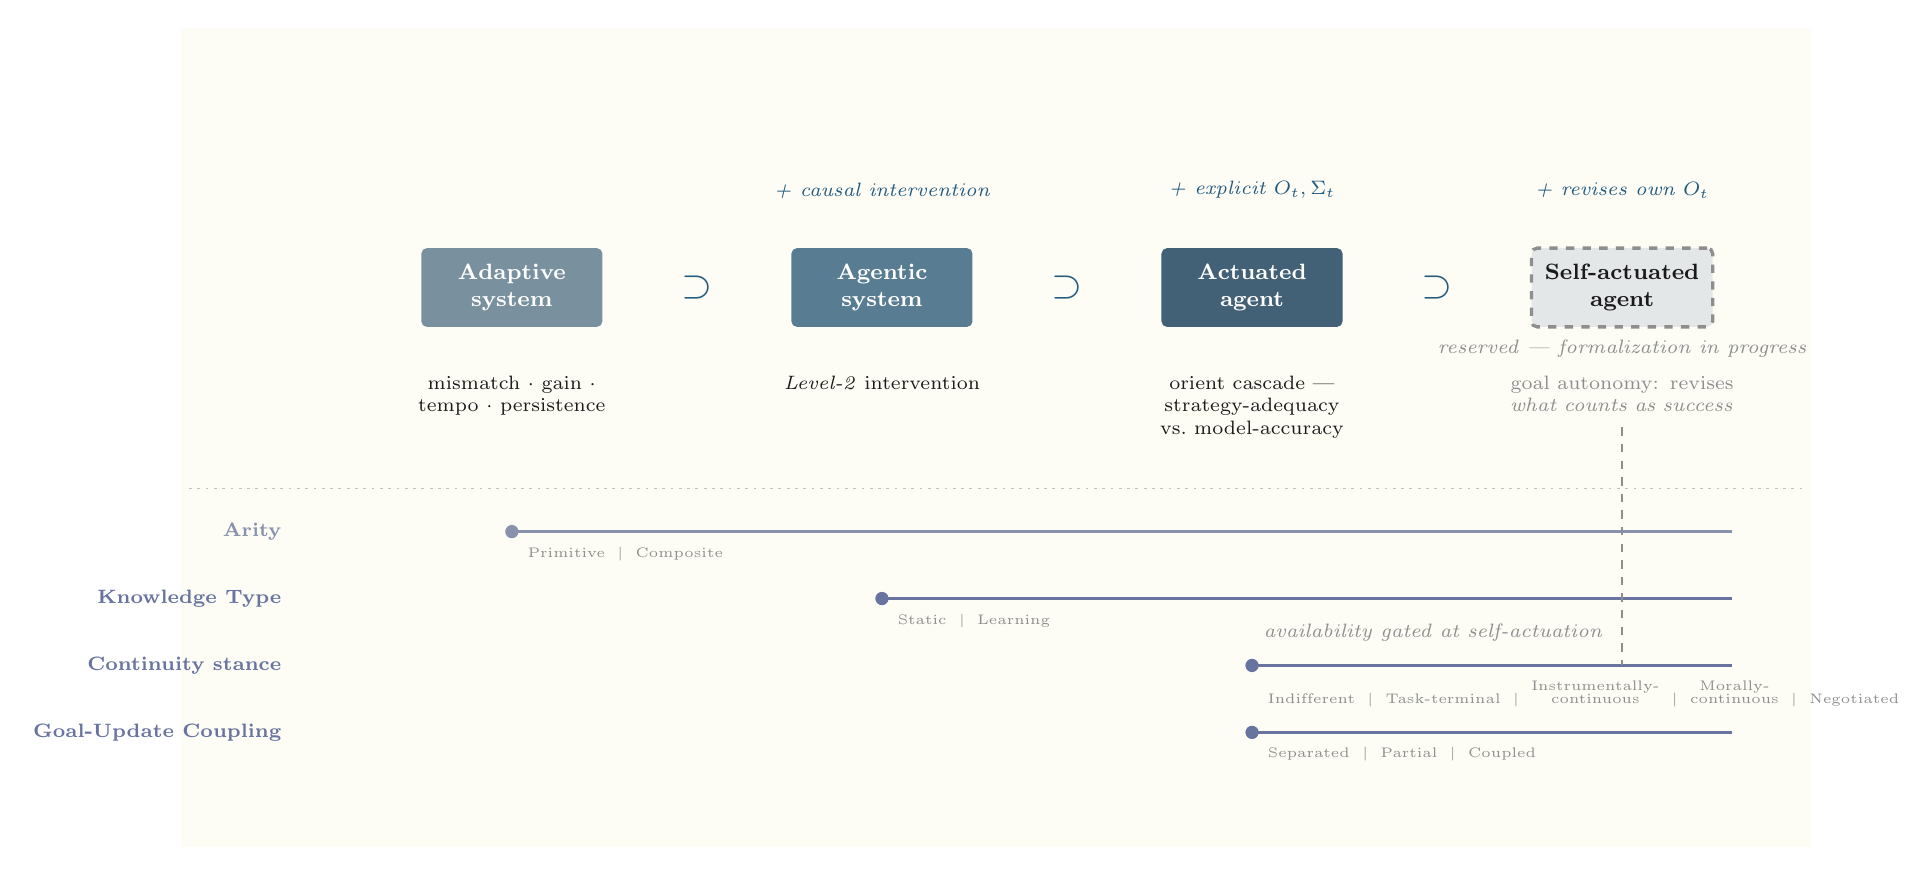
\begin{tikzpicture}[
  font=\small,
  every node/.style={inner sep=2pt},
  station/.style={rectangle, rounded corners=2pt, minimum width=2.3cm,
                  minimum height=1.0cm, align=center, text=white,
                  font=\footnotesize\bfseries},
  reserved/.style={rectangle, rounded corners=2pt, minimum width=2.3cm,
                  minimum height=1.0cm, align=center, text=ink,
                  draw=midgray, dashed, very thick, fill=coolgray!30,
                  font=\footnotesize\bfseries},
  capbox/.style={align=center, text=ink, font=\scriptsize,
                  text width=3.1cm, anchor=north},
  delta/.style={align=center, anchor=south,
                  font=\scriptsize\itshape, text=spineDeep},
  rail/.style={railPeri, line width=1.1pt},
  raillab/.style={text=railPeri, font=\scriptsize\bfseries, anchor=east},
  % discrete choices: small, dimmed, set just BELOW the rule so the
  % rule itself stays clean and continuous (no ground-fill masking)
  railsub/.style={text=midgray, font=\tiny, anchor=north west,
                  inner sep=1pt},
]

\fill[ground] (-3.3,1.0) rectangle (17.4,11.4);

% ===== ZONE 1: definitional-narrowing spine (Vol-1 scope) =====
% Three rows: deltas (what each refinement adds) ABOVE the recipient
% node, the class spine in the middle (clean arrows, no text masking
% the line), capabilities BELOW each node. \sy raised from 6.7 -> 8.1
% to open the band below the spine for the relocated capability row.
\def\sy{8.1}
\def\dx{4.7}
\foreach \i in {0,...,3}{ \pgfmathsetmacro\xx{0.9+\i*\dx}
  \coordinate (S\i) at (\xx,\sy); }

\begin{scope}[on background layer]
  \fill[spineDeep!8]
    ($(S0)+(-1.55,0.95)$) -- ($(S3)+(1.55,0.46)$) --
    ($(S3)+(1.55,-0.46)$) -- ($(S0)+(-1.55,-0.95)$) -- cycle;
\end{scope}

\node[station, fill=spineA]  (n0) at (S0) {Adaptive\\system};
\node[station, fill=spineB]  (n1) at (S1) {Agentic\\system};
\node[station, fill=spineC]  (n2) at (S2) {Actuated\\agent};
\node[reserved]              (n3) at (S3) {Self-actuated\\agent};

\node[text=midgray, font=\scriptsize\itshape, anchor=north]
  at ($(n3.south)+(0,-0.07)$) {reserved --- formalization in progress};

% (C) The spine relation is proper CONTAINMENT, not a process/flow:
% Adaptive (broadest population) supset Agentic supset Actuated supset
% Self-actuated (rarest). A directed arrow misread this as a pipeline;
% the superset glyph is the canonical relation (design doc section 2:
% #scope-adaptive-system \supset #scope-agency). Each box sits inside
% the population of the one to its left.
\foreach \i in {0,1,2}{
  \pgfmathsetmacro\xm{0.9+\i*\dx+\dx/2}
  \node[text=spineDeep, font=\Large] at (\xm,\sy) {$\supset$};}

% Row 1: the increment each refinement adds, parked over the RECIPIENT
% node (the class that increment produces). Adaptive (n0) is the base
% of the spine, so it carries no delta.
\def\dy{9.15}
\node[delta] at (S1|-0,\dy) {+ causal intervention};
\node[delta] at (S2|-0,\dy) {+ explicit $O_t,\Sigma_t$};
\node[delta] at (S3|-0,\dy) {+ revises own $O_t$};

% Row 3: the capability each class buys --- now BELOW its node. The
% old "the capability each refinement buys" header label is dropped:
% the three-row stacking makes the relationship self-evident.
\def\capy{7.05}
\node[capbox] at (S0|-0,\capy) {mismatch $\cdot$ gain $\cdot$ tempo
  $\cdot$ persistence};
\node[capbox] at (S1|-0,\capy) {\emph{Level-2} intervention};
\node[capbox] at (S2|-0,\capy) {orient cascade --- strategy-adequacy
  vs.\ model-accuracy};
\node[capbox, text=midgray] (capS3) at (S3|-0,\capy) {goal autonomy:
  revises \emph{what counts as success}};

% ===== ZONE 2: orthogonal property rails =====
\draw[midgray!55, dash pattern=on 1pt off 2pt] (-3.2,5.55) -- (17.3,5.55);

\def\railR{16.4}
% Each rail: a single clean continuous rule; the switch-on dot marks
% where it activates; the discrete choices sit just BELOW the rule,
% smaller and dimmed (no ground-fill masking the line). The drop is a
% snug ~half-line so each choice group visually binds to its OWN rule
% (the rail directly above it), not to the next rail down.
\def\rsub{-0.15}  % vertical drop of the choice text below each rule

% Rail order (top -> bottom): Arity, Knowledge Type, Continuity
% stance, Goal-Update Coupling. Each rail's switch-on dot sits at the
% tier where the property first becomes meaningful.

% Arity — all tiers (spans full width, on from Adaptive)
\draw[railPeri2, line width=1.1pt] (0.9,5.0) -- (\railR,5.0);
\fill[railPeri2] (0.9,5.0) circle (2.4pt);
\node[raillab, text=railPeri2] at (-1.95,5.0) {Arity};
\node[railsub] at ($(0.9,5.0)+(0.16,\rsub)$) {Primitive $\;\vert\;$
  Composite};

% Knowledge Type — switches on at Agentic
\draw[rail] (S1|-0,4.15) -- (\railR,4.15);
\fill[railPeri] (S1|-0,4.15) circle (2.4pt);
\node[raillab] at (-1.95,4.15) {Knowledge Type};
\node[railsub] at ($(S1|-0,4.15)+(0.16,\rsub)$) {Static $\;\vert\;$
  Learning};

% Continuity stance — orthogonal; availability gated at Self-actuation
\draw[rail] (S2|-0,3.3) -- (\railR,3.3);
\fill[railPeri] (S2|-0,3.3) circle (2.4pt);
\node[raillab] at (-1.95,3.3) {Continuity stance};
\node[railsub] at ($(S2|-0,3.3)+(0.16,\rsub)$) {Indifferent $\;\vert\;$
  Task-terminal $\;\vert\;$ \shortstack{Instrumentally-\\[-2.4pt]continuous}
  $\;\vert\;$ \shortstack{Morally-\\[-2.4pt]continuous} $\;\vert\;$
  Negotiated};
% dashed drop gating this rail at the self-actuation column. Starts
% just BELOW the Self-actuated capability box (capS3) --- since the
% spine moved up and capabilities now sit under their node, anchoring
% to n3.south would run the line straight through that text.
\draw[midgray, dashed, line width=0.85pt]
  ($(capS3.south)+(0,-0.12)$) -- (S3|-0,3.3);
% gate annotation: parked just above this rail, left of the dashed
% self-actuation line, so it clears the choices below
\node[text=midgray, font=\scriptsize\itshape, anchor=east]
  at ($(S3|-0,3.72)+(-0.18,0)$) {availability gated at self-actuation};

% Goal-Update Coupling — switches on at Actuated
\draw[rail] (S2|-0,2.45) -- (\railR,2.45);
\fill[railPeri] (S2|-0,2.45) circle (2.4pt);
\node[raillab] at (-1.95,2.45) {Goal-Update Coupling};
\node[railsub] at ($(S2|-0,2.45)+(0.16,\rsub)$) {Separated $\;\vert\;$
  Partial $\;\vert\;$ Coupled};

\end{tikzpicture}
\end{document}
